\section{Wyniki}



Proponuje tutaj wrzucać zdjęcia, tabele, raczej nie dużo tekstu
WYnik - oprogramowanie i to co wychodzi jako wynik oprogramowania 

\subsection{Gaussian Splatting}
Przy pomocy biblioteki \textit{gsplat} implementującej Gaussian Splatting w Pythonie wykonaliśmy eksperymenty polegające na uruchomeniu algorytmu dla różnych wartości hiperparametrów w celu znalezienia optymalnych dla nich wartości. Poniżej znajdują się wnioski dotyczące znaczenia hiperparametrów na podstawie obserwacji procesów trenowania dla różnych ustawień.

\begin{enumerate}
    \item Liczba Gaussianów: w przypadku scen urbanistycznych w celu oddania odpowieniej szczegółowości potrzebne jest parę milionów Gaussianów, dla naszych scen było to zwykle 3 mln.
    \item Strategia adaptacji: wybór strategii jest istotny gdyż określa sposób dodawania i usuwania Gaussianów oraz wpływa na jakość sceny.
    \item Liczba iteracji: zwykle im dłużej trenowana jest scena tym lepsze wyniki otrzymujemy, jednak zależy to również od przyjętej strategii.
    \item Stopień zmiennych harmonicznych: zmienne harmoniczne wyrażają kolor, im większy stopień tym lepsza jakość sceny, ale też zwiększone zużycie pamięci.  
\end{enumerate}

tutaj zdjecia dla oczkow 

\begin{figure}[!h]
    \centering
    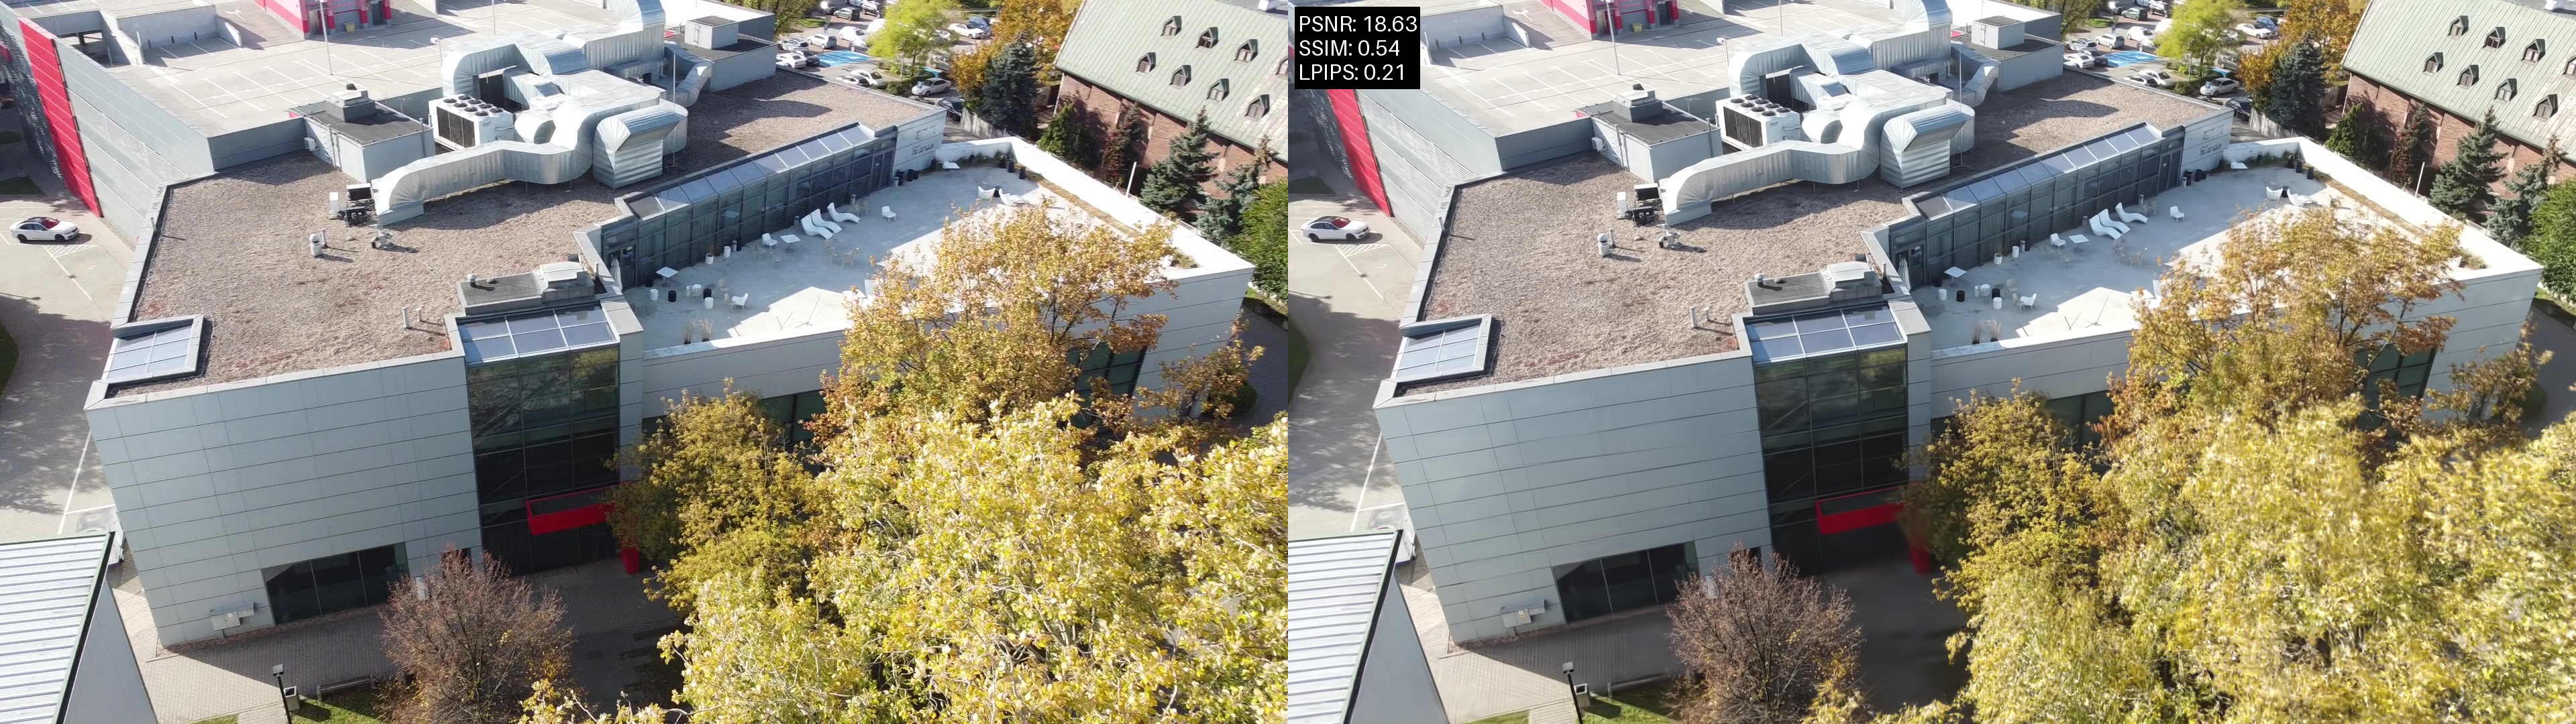
\includegraphics[width=1.0\linewidth]{images/sks_viper_0008.png}
    \caption{Scena SKS (od lewej do prawej: prawdziwe zdjęcie i widok modelu)}
    \label{fig:sks_res_0008}
\end{figure}